\documentclass[12pt]{turabian-researchpaper}
\usepackage{graphicx}
\usepackage{amsmath}
\usepackage{amsfonts}
\usepackage{float}
\usepackage{xcolor}
\usepackage[pass, letterpaper]{geometry}
%\usepackage[notes,backend=biber]{biblatex-chicago}
%\usepackage[authordate,backend=biber]{biblatex-chicago}
%\usepackage[authordate-trad,backend=biber]{biblatex-chicago}
\usepackage[authordate,backend=biber]{biblatex-chicago}
\addbibresource{ai.bib}
\addbibresource{464_final.bib}

\providecommand{\keywords}[1]{\textbf{\textit{Keywords:}} #1}

\title{DRAFT ... Us Versus Stockfish}
\subtitle{Using Nerual Networks to Play Chess}
\author{Philmore Morrison}
\submissioninfo{philmoremorrison2023@u.northwestern.edu}
\date{Nov 18, 2021}
\begin{document}
\maketitle

\begin{abstract}
    \noindent
    We use a deep neural network to learn how to play chess against the famous Stockfish program.\\
\noindent\keywords{Chess, Stockfish, Policy Estimation, Deep Learning}
\end{abstract}

\section*{Introduction}

We survey multiple learning methods for learning policy approximation in reinforcement learning. Our objective is to train a neural network model to play chess. 

\textbf{... add more information to the introduction section.}
\textbf{\\\color{orange}{https://github.com/arjangroen/RLC} \\}  is a great example of the types of agents we can explore.


\section{Literature Review}

A long-standing ambition of artificial intelligence has been to create programs that can instead learn for themselves from first principles \parencite{silver_general_2018}. Researchers have used countless resources in the pursuit of a proficient chess-playing algorithm. Through experience, one might learn to predict whether chess positions will lead to a win \parencite{sutton1988learning}. The game of chess is the longest-studied domain in the history of artificial intelligence \parencite{silver_general_2018}. The seminal works of Claude Shannon, Alan turning, and countless researchers derived the theory and built hardware to play chess efficiently. Chess programs evaluated positions using handcrafted features and carefully tuned weights, constructed by strong human players and programmers, combined with a high-performance alpha-beta search that expands a vast search tree using a large number of clever heuristics and domain-specific adaptations \parencite{silver_general_2018}. Handcrafted heuristics guarantee that subsequent chess algorithms could not be useful outside of the world of chess. There are also too many permutations and moves for humans to hand-code an algorithm effectively. The rules in chess are position and piece dependent. For example, pawns can move two steps forward from the second row (player‘s perspective). The queen can move across the board freely, and under the right circumstances, a player can castle. We can describe a move in chess in two parts. The agent first selects a piece to move, then selects aan action from the possible moves for the chosen piece.

Deep Blue was developed at IBM in the 1990s after multiple years of research and development, focusing on building a world-class chess machine \parencite{campbell_deep_2002}. Deep Blue I lost to Garry Kasparov in 1996, four to two. The Deep Blue team modified the Deep Blue architecture and rechallenged Kasparov again in 1997. Deep Blue defeated Garry Kasparov in the 1997 match by a score of 3.5–2.5, and the  Deep Blue team was awarded the Fredkin prize for defeating the human world champion in a regulation match \parencite{campbell_deep_2002}.

Chess subsequently became a grand challenge task for a generation of artificial intelligence researchers, culminating in high-performance computer chess programs that play at a super-human level \parencite{silver_general_2018}. Monte Carlo Tree Search (MCTS) is one such method. The MCTS algorithm consists of the following phases; selection, expansion, simulation, and backpropagation.  During the selection phase, the algorithm searches the portion of the tree that has already been represented in memory \parencite{swiechowski2021}. Next, the expansion phase is triggered if the selection phase does not reach a terminal state. The expansion adds new nodes corresponding to state s-prime (new-state) based on the previous action. Next, simulation implements the Monte Carlo part of the algorithm to estimate possible reward and terminal state. Finally, backpropagation distributes the simulated scores up the tree to the root node while updating the statistics for visits \(n_i\) and state estimate \(S_i\). 

MCTS has an advantage over traditional depth-limited minimax search with alpha-beta pruning in games with high branching factors such as Go, while minimax search with alpha-beta pruning surpasses MCTS in domains like Chess \parencite{lin_monte_2017}. MCTS does not detect shallow traps as well as minimax search. Missing a shallow trap has the consequence of an opponent winning within a few moves. During minimax search, we build a tree from position \(x\) by examining all possible moves for the computer in that position, then all possible moves for the opponent, followed by all possible moves for the computer to a predetermined depth \(d\) \parencite{baxter_learning_2000}. 

Temporal Difference (TD) learning is another algorithm for learning policies. Arthur Samuel introduced TD learning in 1959. \Textcite{samuel1959} created a checkers playing system based on TD learning. \Textcite{sutton1988learning} contributed to the literature by using TD learning as an incremental learning process for making predictions. TD approximates the expected long-term future cost (or cost-to-go) of a stochastic dynamical system as a function of the current state \parencite{baxter_learning_2000}. The main objective is to minimize the error between the prediction for the current and the next state. TD learning became popular because it combined the advantages of dynamic programming and the Monte Carlo method without the total computational overhead. TD learning also leverages the bootstrap method similar to Dynamic Programming. One significant benefit of TD learning is that we do not need to wait until the end of an episode to compute the \(Q\) value. Said another way, ``TD learning bootstraps like DP, so it does not have to wait till the end of the episode, and like the MC method, it does not require the model dynamics of the environment to compute the value function or the Q function" \parencite{science_understanding_2021}. We provide a visual comparison between MCTS and TD learning in figure \ref{fig:td_mc}. 

\begin{figure}[!ht]
    \centering
    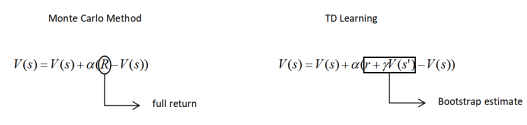
\includegraphics[width=0.95\textwidth]{mcts_td.png}
    \caption{\textit{ Value function based on Monte Carlo tree search versus Temporal Difference learning}}
    \label{fig:td_mc}
\end{figure}

AlphaZero replaces the handcrafted knowledge and domain-specific augmentations used in traditional game-playing programs with deep neural networks, a general-purpose reinforcement learning algorithm, and a general-purpose tree search algorithm \parencite{silver_general_2018}. AlphaZero uses a deep neural network to play chess. The network uses board position as inputs and outputs for move probabilities based on the non-linear evaluations of the board position. AlphaZero learned to approximate the policies through self-play and experience replay based on the Monte Carlo tree search algorithm. AlphaZero can search 60,000 positions per second in chess. \Textcite{silver_general_2018} states that AlphaZero defeated Stockfish when given 1/10 as much thinking time as Stockfish. Stockfish is an open-source chess program that is ranked as the strongest CPU chess engine in the world. 

We leverage the work of the practitioners that came before us to build neural network agents to play chess against the Stockfish chess program. The remainder of this document is as follows. We discuss the training dataset next, followed by our design of experiments, methodologies, and results. Finally, we conclude the paper with our overall findings and discussion for future enhancements. 

\section{Data}

Discuss the data that we use in the experiments ... experience replay (self-play) or against an opponent (Stockfish). Elo range for 'training'.


\section{Methods \& Results}

We conduct a series of experiments using different network topologies. Our agent competes against Stockfish. We need to frame the problem and produce some plots to include in the final presentation.  

\subsection{Experiment One}

Exp one is ...

\subsection{Experiment One}

Exp two goes burrrrrr ...

\section{Conclusion \& Future Works}

In closing, our results show ... blah blah blah

Future considerations include parallel or multi-processing during training or leveraging REINFORCE or Actor-Critic methods.

\clearpage
\printbibliography[title={References}]
\end{document}

